\documentclass[10pt,a4paper]{beamer}
\usepackage[utf8]{inputenc}
\usepackage[portuguese]{babel}
\usepackage[T1]{fontenc}
\usepackage{amsmath}
\usepackage{amsfonts}
\usepackage{amssymb}
\begin{document}
\section{Propriedades dos termos do Near-Fields}

\begin{frame}

\frametitle {Propriedades dos termos do Near-Field}

\begin{itemize}
\item Definimos o campo de deslocamento próximo $u^{N}$ por:
\end{itemize}

\begin{equation}
u_{i}^{N}(x,t)= \frac{1}{4\pi\rho}(3\gamma_{i}\gamma_{j}-\delta_{ij})\frac{1}{r^{3}} \int_{r/\alpha}^{r/\beta} \tau X_{0}(t-\tau) \,d\tau\ .
\end{equation}

\begin{figure}
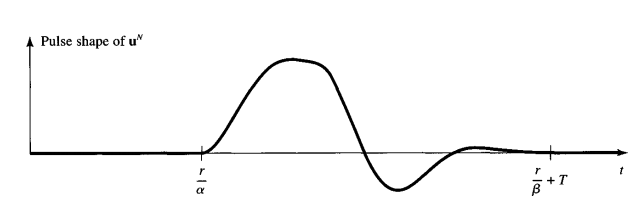
\includegraphics[scale=1.5]{fig1.png}
\end{figure}


\end{frame}

\begin{frame}
\begin{itemize}
\item componente longitudinal

\begin{equation}
u^{N}.\gamma= \gamma _{j}\frac{1}{2\pi\rho r^{3}}\int_{r/\alpha}^{r/\beta} \tau X_{0}(t-\tau) \,d\tau\ .
\end{equation}

\item componente transversal
\begin{equation}
u^{N}.\gamma^{'}= -\gamma^{'} _{j}\frac{1}{4\pi\rho r^{3}}\int_{r/\alpha}^{r/\beta} \tau X_{0}(t-\tau) \,d\tau\ .
\end{equation}
\end{itemize}


\end{frame}

\begin{frame}
\frametitle {Near-Field (Campos próximos)}
\begin{itemize}
\item Para o deslocamento Near-Field, não é possível identificar as propriedades simples como nos campos distantes; 
\item Podemos identificar o tempo de transito e a duração do deslocamento em um receptor fixo;
\item A duração do movimento do campo de deslocamento Near Field é igual a diferença entre os tempos de transitos das ondas P e S mais o termo T.
\end{itemize}
\end{frame}


\end{document}